\section{Исследование рынка} \label{economics_market_research}

В разрабатываемом ПО в первую очередь заинтересованы организации, желающие внедрить систему электронного документооборота, одним из направлений деятельности которых является инженерия программного обеспечения.
Только среди компаний, занимающихся вопросами информационной безопасности, обладателей лицензии ФСТЭК на деятельность по разработке и производству средств защиты конфиденциальной информации более тысячи, не считая лицензиатов ФСБ, Минобороны.
Общее число предприятий, осуществляющих разработку программного обеспечения в разных областях, составляет не менее 3 000.

\vspace{\baselineskip}
На рынке существуют аналоги разрабатываемого ПО. Компания <<Логика бизнеса 2.0>> разрабатывает систему электронного документооборота <<Логика ЕСМ. СЭД>>, являющуюся частью комплексного решения <<Логика ЕСМ>> и основанную на платформах IBM Collaboration Solution (Lotus Notes/Domino) и СПО. Однако в качестве клиентского ПО под Linux предлагается Web-доступ, что несовместимо со средствами криптографической защиты информации, применяемыми для работы с электронной подписью. Кроме того, данная система является одной из самых дорогих --- от 350 000 руб. для группы из 20 пользователей.

Другие системы, представленные на российском рынке (LanDocs, DIRECTUM, OPTIMA, и т.д.) обладают схожими недостатками --- отсутствие полноценных клиентов под свободные платформы (поддерживается только Windows), отсутствие сертификатов ФСТЭК, отсутствие внятно декларированной системы доверенного хранения истории изменений документов.

Более подробный анализ существующих решений представлен в исследовательской части.

\vspace{\baselineskip}
Учитывая количество заинтересованных организаций, оценим число потенциальных покупателей на годовом интервале времени $N_P^O = 60$.

\subsection{Планирование цены и прогнозирование прибыли} \label{pricing}

<<Рыночную>> стоимость ПО можно рассчитать, используя соотношение (\ref{eq:market_cost}):
\begin{equation}
  \label{eq:market_cost}
K_\textrm{ПР} = (\Delta K + K_\textrm{ВН}) + \cdot (1 + D_\textrm{ПРИБ}),
\end{equation}
где $\Delta K$ --- часть стоимости разработки, приходящаяся на одну копию программы, $K_\textrm{ВН}$ --- стоимость внедрения программы, $D_\textrm{ПРИБ}$ --- процент прибыли, заложенный в стоимость.

\vspace{\baselineskip}
Частичная стоимость разработки, приходящаяся на каждый комплект ПО, определяется исходя из данных о планируемом объеме установок:
\begin{equation}
  \label{eq:item_cost}
\Delta K = \frac {K} {N_P} \cdot (1 + H_\textrm{СТ}),
\end{equation}
где $K$ --- стоимость проекта, $N_P$ --- планируемое число копий ПО, $H_\textrm{СТ}$ --- ставка банковского процента по долгосрочным кредитам (более одного года).

\vspace{\baselineskip}
Приняв ставку процента по долгосрочным кредитам 21\% (ЗАО КБ <<Ситибанк>>) и используя полученные ранее значения, вычислим:
\begin{equation}
  \label{eq:item_cost_calculate}
\Delta K = \frac {545871,29} {60} \cdot (1 + 0,21) = 9097,85 \cdot 1,21 = 11008,40 \textrm{ (руб.)}
\end{equation}

Установим $K_\textrm{ПР} = 40 000$ рублей. Данная стоимость ниже среднерыночной, что позволит привлечь б\textit{о}льшее число покупателей.

\vspace{\baselineskip}
Тем самым, сумма от продаж за год составит $60 \cdot 40 000 = 2400000$ рублей, что обесечивает срок окупаемости проекта менее 1 года.

Определим процент прибыли от одной реализации ПО по формуле:
\begin{equation}
  \label{eq:profit}
D_\textrm{ПРИБ} = (\frac {K_\textrm{ПР}} {\Delta K + K_\textrm{ВН}} - 1) \cdot 100 ,
\end{equation}
где $K_\textrm{ВН} = 0$ --- затраты на внедрение.

\vspace{\baselineskip}
Для данного проекта:
\begin{equation}
  \label{eq:profit_calc}
D_\textrm{ПРИБ} = (\frac {40 000} {11 008,40} - 1) \cdot 100 = 363,36.
\end{equation}

% \vspace{\baselineskip}
Сумма расчётной прибыли от продажи каждой установки ПО с учётом налога на добавочную стоимость $H_\textrm{НДС} = 18\%$:
\begin{equation}
  \label{eq:clear_profit}
C_\textrm{ПРИБ} = (\Delta K + K_\textrm{ВН}) \cdot D_\textrm{ПРИБ} \cdot (1 - H_\textrm{НДС}) = 11008,40 \cdot 3,6336 \cdot 0,82 = 32800,10 \textrm{ (руб.)}
\end{equation}

Для оплаты расходов на разработку ПО возьмем кредит в банке ЗАО КБ <<Ситибанк>> в размере 650000 рублей на срок 24 месяца. Ежемесячный платеж по данному кредиту составляет 33401 руб. Сумма погашения кредита (с учётом комиссии за обслуживание кредита) составляет 801624 рублей.

За первые три месяца разработки продажи равны нулю, т.к. продукт еще не разработан. При этом осуществляются выплаты заработной платы и производятся другие ранее рассчитанные расходы на разработку в размере 545871,29 рублей.

Будем считать, что через три месяца после начала разработки за каждый последующий год продается 60 экземпляров программы (5 в месяц).

Фрагмент таблицы общего баланса приведен в таблице \ref{table:balance}. Из таблицы видно, что в августе 2014 года возможно досрочное погашение кредита. Структура дохода показана на рисунке \ref{img:income_structure}.

\begin{table} [h!]
  \captionsetup{justification=raggedright}
  \caption{Фрагмент таблицы общего баланса}\label{table:balance}
 \begin{center}
  \begin{tabular}{| >{\centering}m{2cm} | >{\centering}m{2cm} | >{\centering}m{2cm} | >{\centering}m{2cm} | >{\centering}m{2cm} | >{\centering}m{2cm} | >{\centering}m{2cm} |}
  \hline
 \rowcolor{Gray} Период расчёта  & Баланс начальный, руб. & Сумма продаж, руб. & Расход (включая сумму погашения кредита), руб. &  Чистая прибыль, руб. & Баланс конечный, руб. & Остаток по кредиту, руб. \tabularnewline \hline

02-04.2014 & 650000,00 & 0,00 & 646074,29 & -646074,29 & 3925,71 & 701421,00 \tabularnewline \hline
05.2014 & 3925,71 & 200000,00 & 33401,00 & 166599,00 & 170524,71 & 668020,00 \tabularnewline \hline
06.2014 & 170524,71 & 200000,00 & 33401,00 & 166599,00 & 337123,71 & 634619,00 \tabularnewline \hline
07.2014 & 337123,71 & 200000,00 & 33401,00 & 166599,00 & 503722,71 & 601218,00 \tabularnewline \hline
08.2014 & 503722,71 & 200000,00 & 33401,00 & 166599,00 & 670231,71 & 567817,00 \tabularnewline \hline

   \end{tabular}
 \end{center}
\end{table}

\begin{figure} [h!] 
  \center
  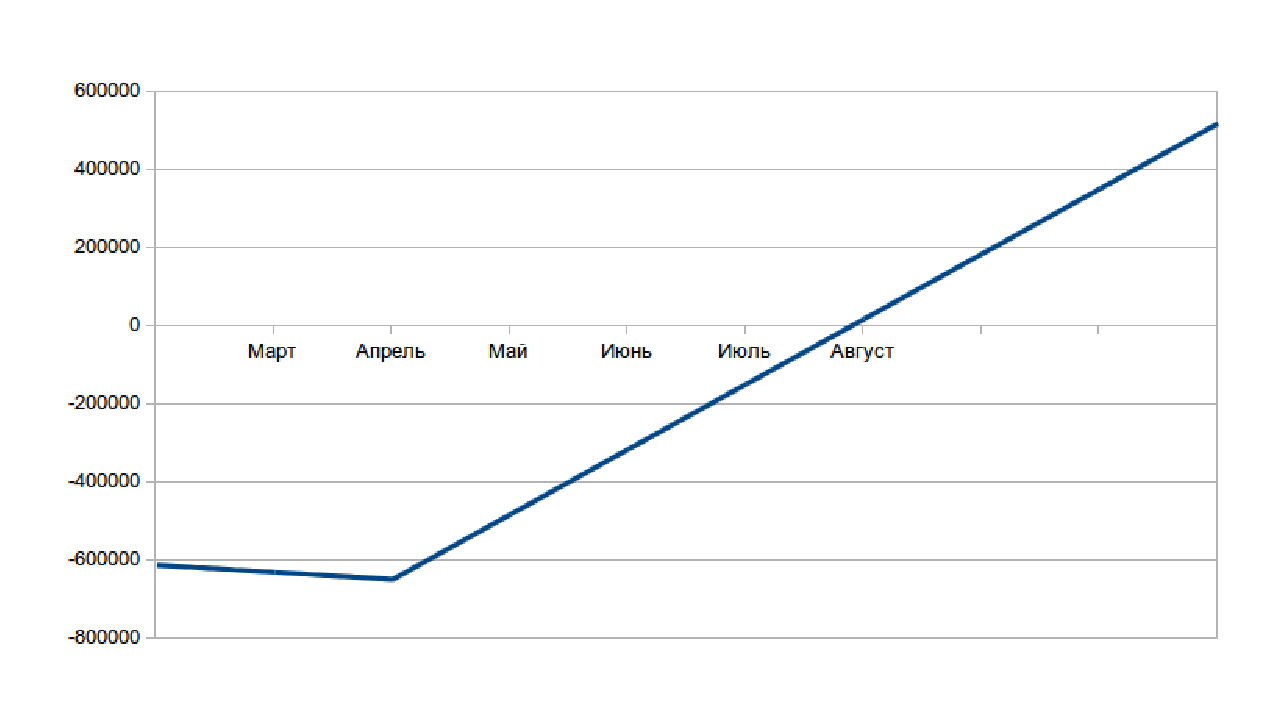
\includegraphics [scale=0.6] {income}
  \caption{Структура дохода} 
  \label{img:income_structure}  
\end{figure}

Таким образом, на графике видно, что срок окупаемости составляет 7 месяцев.           	% Планирование цены и прогнозирование прибыли
\input{economics/economics_service} 	% Сервисное обслуживание
\subsection{Отчисления на социальные нужды} \label{service_social_fee}

Согласно нормативным документам суммарные отчисления в  пенсионный фонд, фонд социального страхования и фонды обязательного медицинского страхования составляют 30\% от размеров заработной платы.
\begin{equation}
  \label{eq:salary_taxes}
C_\textrm{З.ОТЧ} = 0.3 \cdot (C_\textrm{З.ОСН} + C_\textrm{З.ДОП}) = 0.3 \cdot (163373,40 + 32674,68) = 58814,42 \textrm{ руб.}
\end{equation}

Общие расходы на сервисное обслуживание составляют:
\begin{equation}
  \label{eq:salary_sum}
C_\textrm{ЗАРП} = C_\textrm{З.ОСН} + C_\textrm{З.ДОП} + C_\textrm{З.ОТЧ} = 163373,40 + 32674,68 + 58814,42 =  254862,50 \textrm{ руб.}
\end{equation} 	% Отчисления на социальные нужды